\documentclass[11pt,a4paper]{article}
\newcommand{\intestazione}{Trimero ad anello --- 4. Correlatori}
% =====================================================================
%  Preambolo comune ai documenti sul dimero (serie "che cosa abbiamo fatto")
%  Incluso con % =====================================================================
%  Preambolo comune ai documenti sul dimero (serie "che cosa abbiamo fatto")
%  Incluso con % =====================================================================
%  Preambolo comune ai documenti sul dimero (serie "che cosa abbiamo fatto")
%  Incluso con \input{preambolo_dimero} subito dopo \documentclass.
% =====================================================================
\usepackage[T1]{fontenc}
\usepackage[utf8]{inputenc}
\usepackage[main=italian,provide=*]{babel}
\usepackage{amsmath,amssymb,mathtools}
\usepackage{graphicx}
\usepackage{booktabs}
\usepackage{colortbl}
\usepackage{xcolor}
\usepackage{geometry}
\usepackage{placeins}
\usepackage{caption}
\usepackage{enumitem}
\usepackage{fancyhdr}
\usepackage{needspace}
\usepackage{tikz}
\usetikzlibrary{arrows.meta,positioning,shapes.geometric,calc,fit,backgrounds}
\usepackage{hyperref}
\hypersetup{colorlinks=true,linkcolor=blu,citecolor=blu,urlcolor=blu}

\geometry{margin=2.5cm}

% --- colori coerenti con quelli delle figure (palette Okabe-Ito)
\definecolor{blu}{HTML}{0072B2}
\definecolor{arancio}{HTML}{E69F00}
\definecolor{verdes}{HTML}{009E73}
\definecolor{rossos}{HTML}{D55E00}
\definecolor{violas}{HTML}{CC79A7}
\definecolor{grigetto}{HTML}{E8E8E8}

\captionsetup{font=small,labelfont=bf,width=0.92\textwidth}

\pagestyle{fancy}
\fancyhf{}
\fancyhead[L]{\small\itshape\intestazione}
\fancyhead[R]{\small\thepage}
\renewcommand{\headrulewidth}{0.3pt}

% --- notazione
\newcommand{\ket}[1]{\lvert #1\rangle}
\newcommand{\bra}[1]{\langle #1 \rvert}
\newcommand{\media}[1]{\langle #1 \rangle}
\newcommand{\vs}[1]{\mathbf{s}_{#1}}

% --- riquadro "in una riga": il messaggio da portare a casa
\newcommand{\messaggio}[1]{%
  \begin{center}
  \begin{minipage}{0.93\textwidth}
  \setlength{\fboxsep}{9pt}%
  \colorbox{grigetto}{\begin{minipage}{\dimexpr\textwidth-2\fboxsep}
  \small\textbf{In una riga.}\enspace #1
  \end{minipage}}
  \end{minipage}
  \end{center}
}

% --- riquadro "come lo sappiamo": la verifica numerica dietro un'affermazione
\newcommand{\verifica}[1]{%
  \begin{center}
  \begin{minipage}{0.93\textwidth}
  \small\textcolor{verdes}{\rule{2.2em}{1.1pt}}\enspace
  \textcolor{verdes}{\textbf{Come lo sappiamo.}}\enspace #1
  \end{minipage}
  \end{center}
  \medskip
}
 subito dopo \documentclass.
% =====================================================================
\usepackage[T1]{fontenc}
\usepackage[utf8]{inputenc}
\usepackage[main=italian,provide=*]{babel}
\usepackage{amsmath,amssymb,mathtools}
\usepackage{graphicx}
\usepackage{booktabs}
\usepackage{colortbl}
\usepackage{xcolor}
\usepackage{geometry}
\usepackage{placeins}
\usepackage{caption}
\usepackage{enumitem}
\usepackage{fancyhdr}
\usepackage{needspace}
\usepackage{tikz}
\usetikzlibrary{arrows.meta,positioning,shapes.geometric,calc,fit,backgrounds}
\usepackage{hyperref}
\hypersetup{colorlinks=true,linkcolor=blu,citecolor=blu,urlcolor=blu}

\geometry{margin=2.5cm}

% --- colori coerenti con quelli delle figure (palette Okabe-Ito)
\definecolor{blu}{HTML}{0072B2}
\definecolor{arancio}{HTML}{E69F00}
\definecolor{verdes}{HTML}{009E73}
\definecolor{rossos}{HTML}{D55E00}
\definecolor{violas}{HTML}{CC79A7}
\definecolor{grigetto}{HTML}{E8E8E8}

\captionsetup{font=small,labelfont=bf,width=0.92\textwidth}

\pagestyle{fancy}
\fancyhf{}
\fancyhead[L]{\small\itshape\intestazione}
\fancyhead[R]{\small\thepage}
\renewcommand{\headrulewidth}{0.3pt}

% --- notazione
\newcommand{\ket}[1]{\lvert #1\rangle}
\newcommand{\bra}[1]{\langle #1 \rvert}
\newcommand{\media}[1]{\langle #1 \rangle}
\newcommand{\vs}[1]{\mathbf{s}_{#1}}

% --- riquadro "in una riga": il messaggio da portare a casa
\newcommand{\messaggio}[1]{%
  \begin{center}
  \begin{minipage}{0.93\textwidth}
  \setlength{\fboxsep}{9pt}%
  \colorbox{grigetto}{\begin{minipage}{\dimexpr\textwidth-2\fboxsep}
  \small\textbf{In una riga.}\enspace #1
  \end{minipage}}
  \end{minipage}
  \end{center}
}

% --- riquadro "come lo sappiamo": la verifica numerica dietro un'affermazione
\newcommand{\verifica}[1]{%
  \begin{center}
  \begin{minipage}{0.93\textwidth}
  \small\textcolor{verdes}{\rule{2.2em}{1.1pt}}\enspace
  \textcolor{verdes}{\textbf{Come lo sappiamo.}}\enspace #1
  \end{minipage}
  \end{center}
  \medskip
}
 subito dopo \documentclass.
% =====================================================================
\usepackage[T1]{fontenc}
\usepackage[utf8]{inputenc}
\usepackage[main=italian,provide=*]{babel}
\usepackage{amsmath,amssymb,mathtools}
\usepackage{graphicx}
\usepackage{booktabs}
\usepackage{colortbl}
\usepackage{xcolor}
\usepackage{geometry}
\usepackage{placeins}
\usepackage{caption}
\usepackage{enumitem}
\usepackage{fancyhdr}
\usepackage{needspace}
\usepackage{tikz}
\usetikzlibrary{arrows.meta,positioning,shapes.geometric,calc,fit,backgrounds}
\usepackage{hyperref}
\hypersetup{colorlinks=true,linkcolor=blu,citecolor=blu,urlcolor=blu}

\geometry{margin=2.5cm}

% --- colori coerenti con quelli delle figure (palette Okabe-Ito)
\definecolor{blu}{HTML}{0072B2}
\definecolor{arancio}{HTML}{E69F00}
\definecolor{verdes}{HTML}{009E73}
\definecolor{rossos}{HTML}{D55E00}
\definecolor{violas}{HTML}{CC79A7}
\definecolor{grigetto}{HTML}{E8E8E8}

\captionsetup{font=small,labelfont=bf,width=0.92\textwidth}

\pagestyle{fancy}
\fancyhf{}
\fancyhead[L]{\small\itshape\intestazione}
\fancyhead[R]{\small\thepage}
\renewcommand{\headrulewidth}{0.3pt}

% --- notazione
\newcommand{\ket}[1]{\lvert #1\rangle}
\newcommand{\bra}[1]{\langle #1 \rvert}
\newcommand{\media}[1]{\langle #1 \rangle}
\newcommand{\vs}[1]{\mathbf{s}_{#1}}

% --- riquadro "in una riga": il messaggio da portare a casa
\newcommand{\messaggio}[1]{%
  \begin{center}
  \begin{minipage}{0.93\textwidth}
  \setlength{\fboxsep}{9pt}%
  \colorbox{grigetto}{\begin{minipage}{\dimexpr\textwidth-2\fboxsep}
  \small\textbf{In una riga.}\enspace #1
  \end{minipage}}
  \end{minipage}
  \end{center}
}

% --- riquadro "come lo sappiamo": la verifica numerica dietro un'affermazione
\newcommand{\verifica}[1]{%
  \begin{center}
  \begin{minipage}{0.93\textwidth}
  \small\textcolor{verdes}{\rule{2.2em}{1.1pt}}\enspace
  \textcolor{verdes}{\textbf{Come lo sappiamo.}}\enspace #1
  \end{minipage}
  \end{center}
  \medskip
}


\title{\bfseries Misurare una correlazione fra due istanti diversi\\[2pt]
\large Documento 4 --- correlatori dinamici, quattro qubit, 81 combinazioni}
\author{Samuele Schiavi \\ \small Tesi triennale in Fisica, Università di Parma
--- Relatore: Prof.\ Alessandro Chiesa}
\date{}

\begin{document}
\maketitle
\thispagestyle{fancy}

\section{Che cosa vogliamo misurare}

Stessa grandezza del dimero, estesa a tre siti:
\begin{equation}
C_{ij}^{\alpha\beta}(t) = \bra{\psi_0}\,\sigma_i^\alpha(t)\,\sigma_j^\beta(0)\,\ket{\psi_0},
\qquad \alpha,\beta\in\{x,y,z\},\quad i,j\in\{1,2,3\}.
\end{equation}
Con tre siti e tre componenti le combinazioni non sono più $36$ ma
\textbf{81}. Stesso ostacolo di misura del dimero: il prodotto non è
hermitiano, serve un qubit ausiliario.

\section{Il circuito: quattro qubit, non tre}

Stesso schema Hadamard test del dimero, con un registro più grande: tre
qubit fisici più l'ancilla, quattro in tutto. Convenzione ereditata dalla
Parte 1 dell'anello: l'ancilla è il qubit $3$ (non il qubit $0$, come
invece sul dimero) --- un dettaglio di indicizzazione che conta quando si
misura, non solo quando si disegna il circuito.

\begin{figure}[htbp]
\centering
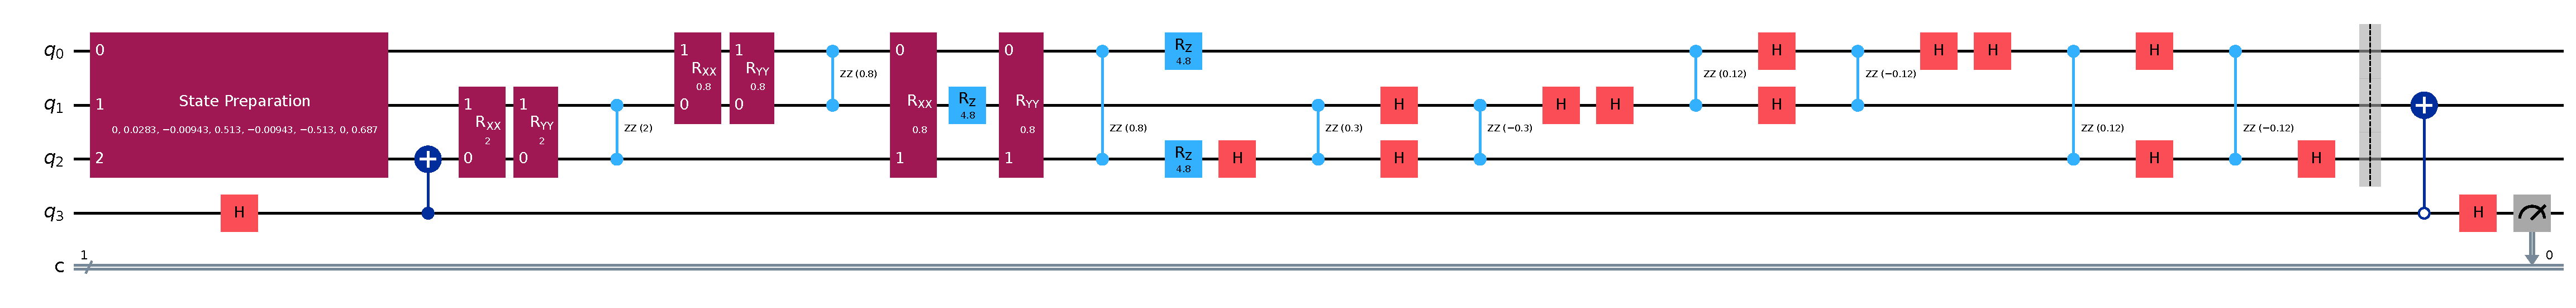
\includegraphics[width=\textwidth]{figure/circ_correlatore_anello_re}
\\[6pt]
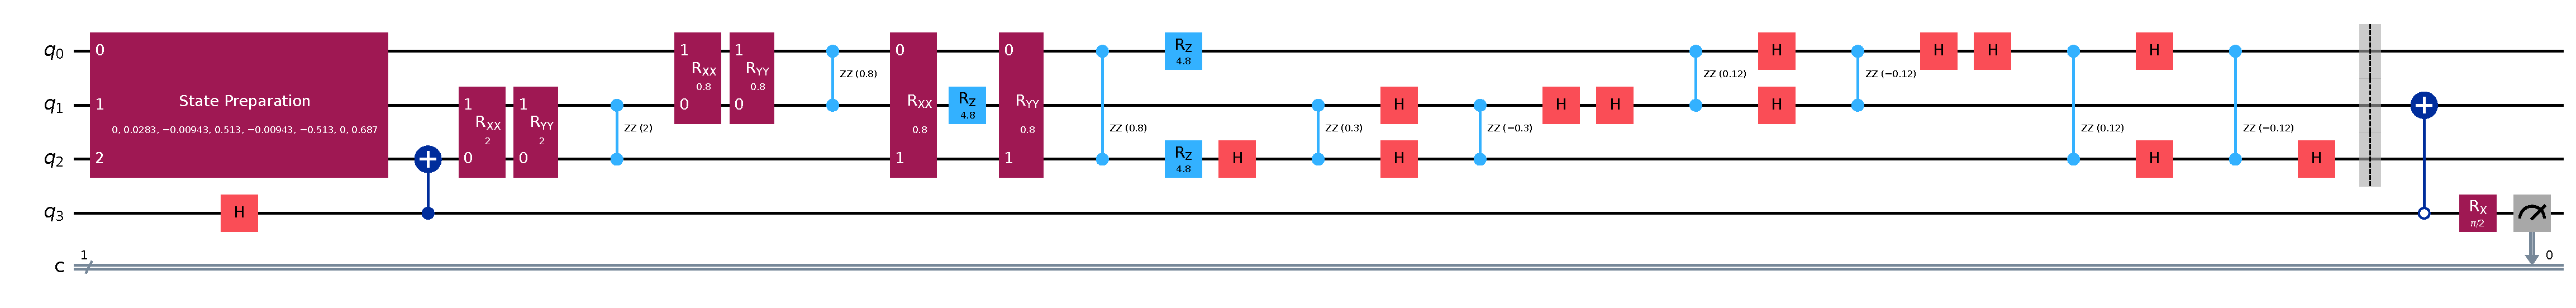
\includegraphics[width=\textwidth]{figure/circ_correlatore_anello_im}
\caption{Il circuito per $C_{21}^{xx}(t{=}1)$, con $N=1$ passo di Trotter
per leggibilità (nell'uso reale, $N=60$), comprensivo del blocco di
misura. \textbf{Sopra}: parte reale. \textbf{Sotto}: parte immaginaria ---
identico fino alla rotazione finale sull'ancilla: $H$ per la parte reale,
$R_x(\pi/2)$ per l'immaginaria. Nell'ordine: preparazione dello stato
fondamentale esatto sul registro a tre qubit (ampiezze dirette, non il
circuito $W$-2q.6 --- coerente con il resto di questo documento);
Hadamard sull'ancilla; $\sigma_1^x$ \textbf{controllata} (pallino pieno,
subito dopo l'Hadamard --- è $\sigma_j^\beta$ con $j{=}1,\beta{=}x$);
evoluzione $U(t)$ non controllata (il blocco di Trotter del Documento 3,
applicato al solo registro); $\sigma_2^x$ \textbf{anti-controllata}
(pallino vuoto, subito dopo l'evoluzione --- è $\sigma_i^\alpha$ con
$i{=}2,\alpha{=}x$); rotazione di base finale e misura dell'ancilla.}
\label{fig:circ-correlatore}
\end{figure}
\FloatBarrier

\section{Verifica: il circuito misura la cosa giusta}

\begin{figure}[htbp]
\centering
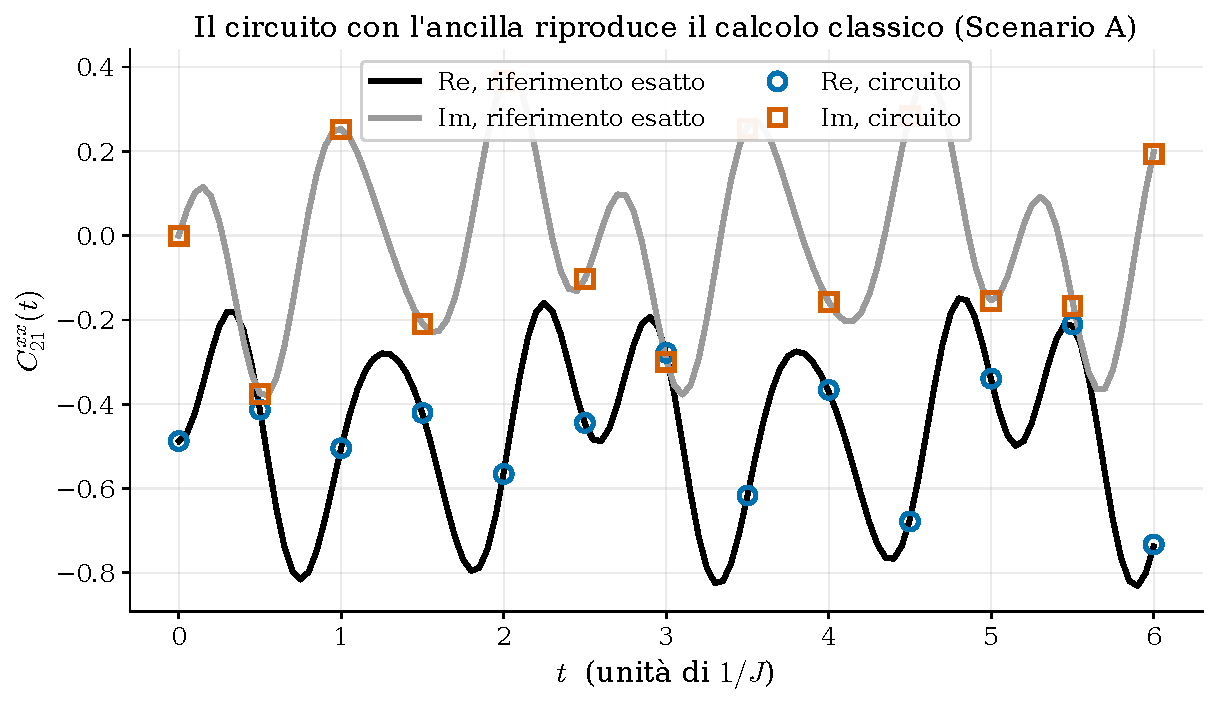
\includegraphics[width=0.86\textwidth]{figure/fig07_correlatore_validazione_anello}
\caption{$C_{21}^{xx}(t)$ al punto Scenario A, riferimento classico
(esponenziale di matrice diretto) contro circuito quantistico ($N=60$).}
\end{figure}
\FloatBarrier

\verifica{Riferimento classico calcolato con implementazione indipendente
(esponenziale di matrice diretto, nessun codice condiviso col circuito).
Confrontato coi valori del circuito su 13 istanti: coincidenza visiva su
tutto l'intervallo mostrato, coerente con l'errore di Trotter atteso a
$N=60$ (Documento 3).}

\section{Lo scan sistematico: 81 combinazioni}

\begin{figure}[htbp]
\centering
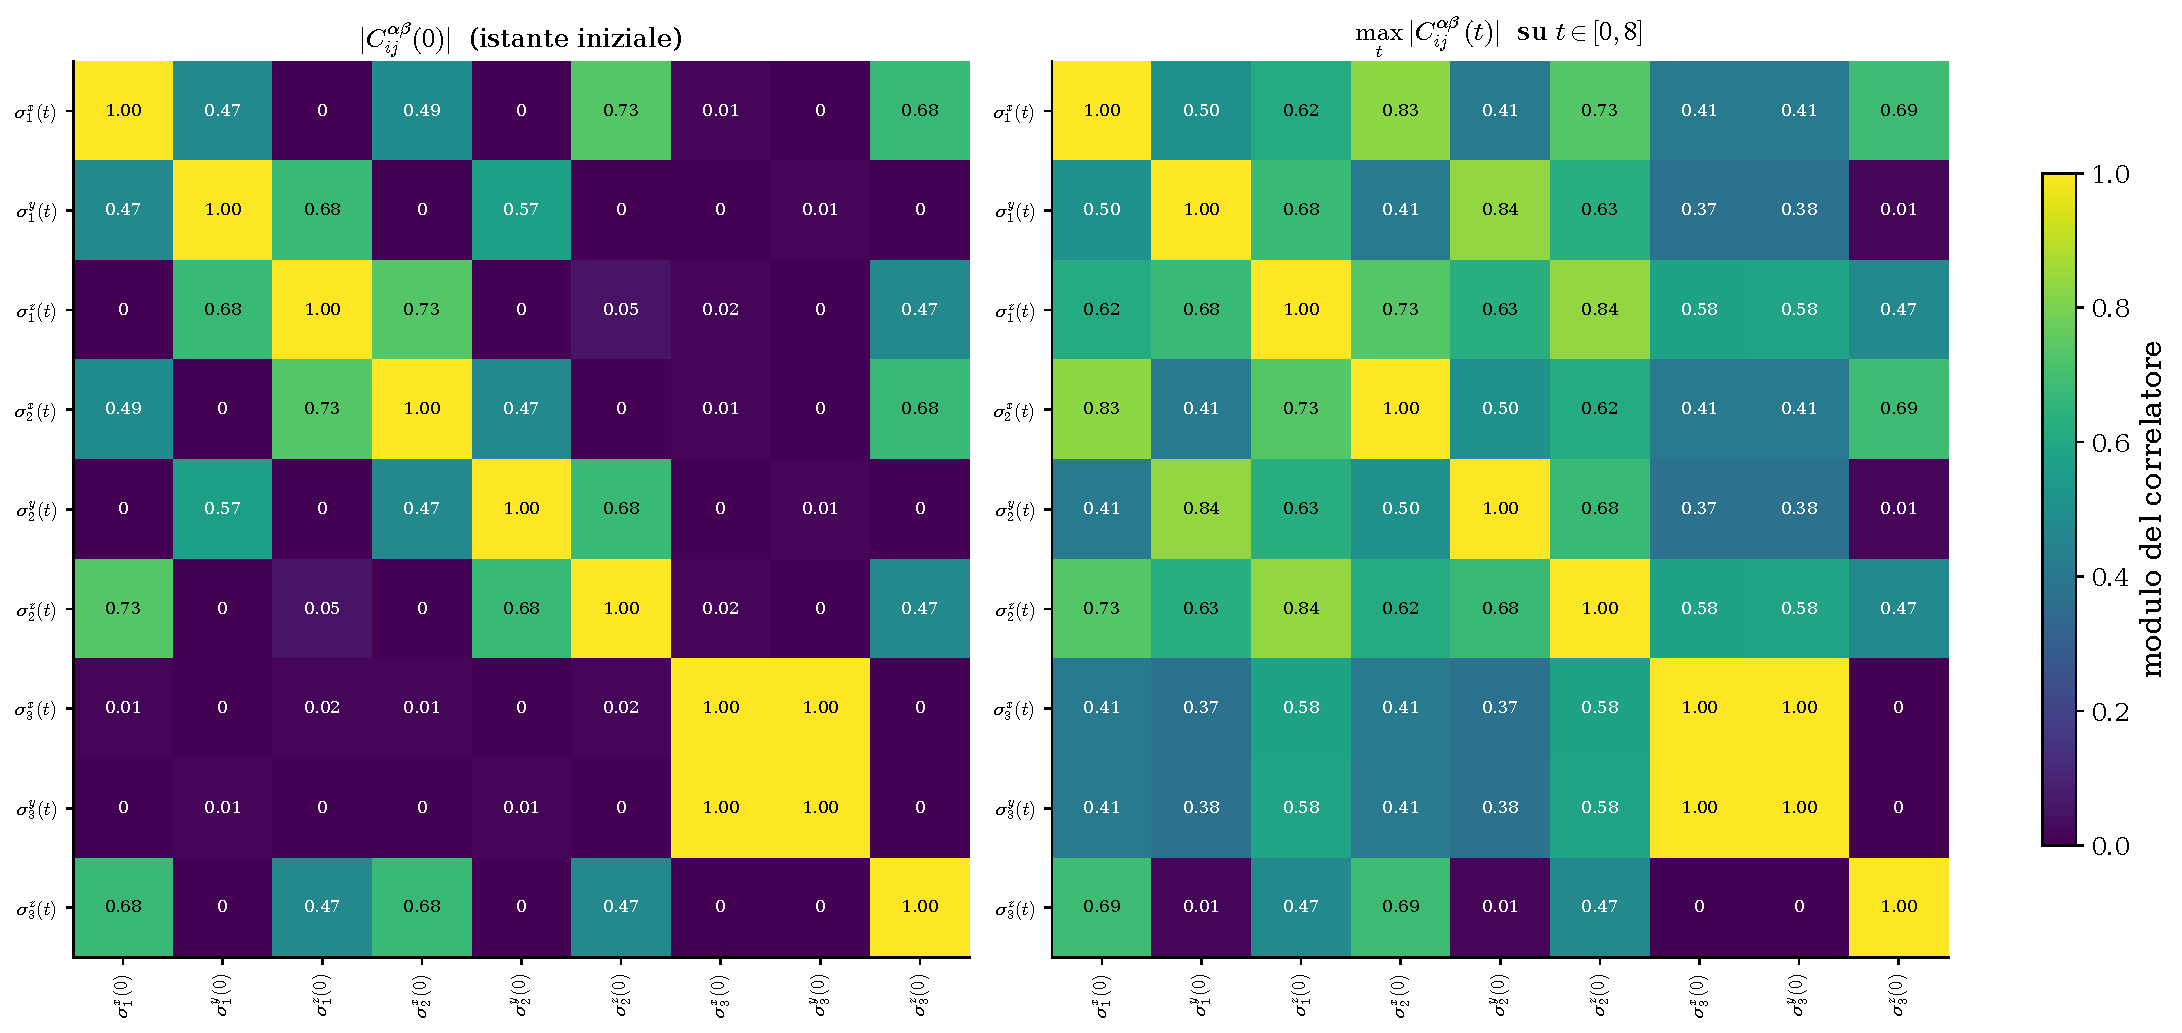
\includegraphics[width=\textwidth]{figure/fig08_scan81_anello}
\caption{Tutte le 81 combinazioni al punto Scenario A. \textbf{Sinistra}:
valore all'istante iniziale. \textbf{Destra}: ampiezza massima su
$t\in[0,8]$. Il confronto fra i due pannelli è il risultato: molte caselle
nulle a $t=0$ (32 su 81) smettono di esserlo appena il sistema evolve ---
solo quattro restano \textbf{esattamente nulle per ogni $t$}
($C_{33}^{xz}$, $C_{33}^{yz}$, $C_{33}^{zx}$, $C_{33}^{zy}$, tutte sullo
stesso sito).}
\label{fig:scan}
\end{figure}
\FloatBarrier

Lo stesso argomento del dimero spiega gli zeri a $t=0$: l'Hamiltoniana è
reale e simmetrica, quindi il fondamentale si può scegliere reale; un
prodotto $\sigma_i^\alpha\sigma_j^\beta$ puramente immaginario ha media
nulla su uno stato reale. Per i \textbf{quattro zeri strutturali} (validi
per ogni $t$, non solo $t=0$) serve qualcosa in più della sola realtà
dell'operatore: sono tutti prodotti sullo stesso sito ($i=j=3$) con
componenti diverse fra $\{x,y,z\}$, ma non tutte le combinazioni
sito-uguale-componenti-diverse sono nulle (per esempio $C_{11}^{xy}$ non lo
è) --- un effetto specifico del sito 3 in questa parametrizzazione
isoscele, verificato numericamente ma non ancora derivato in forma chiusa
in questo pacchetto.

\verifica{Zeri a $t=0$: 32 su 81, verificati a precisione machina
($<10^{-10}$). Zeri strutturali (ampiezza massima nulla su tutto
$t\in[0,8]$, griglia a 81 punti): esattamente 4, lo stesso sottoinsieme
elencato sopra.}

\section{Ricco e monocromatico}

\begin{figure}[htbp]
\centering
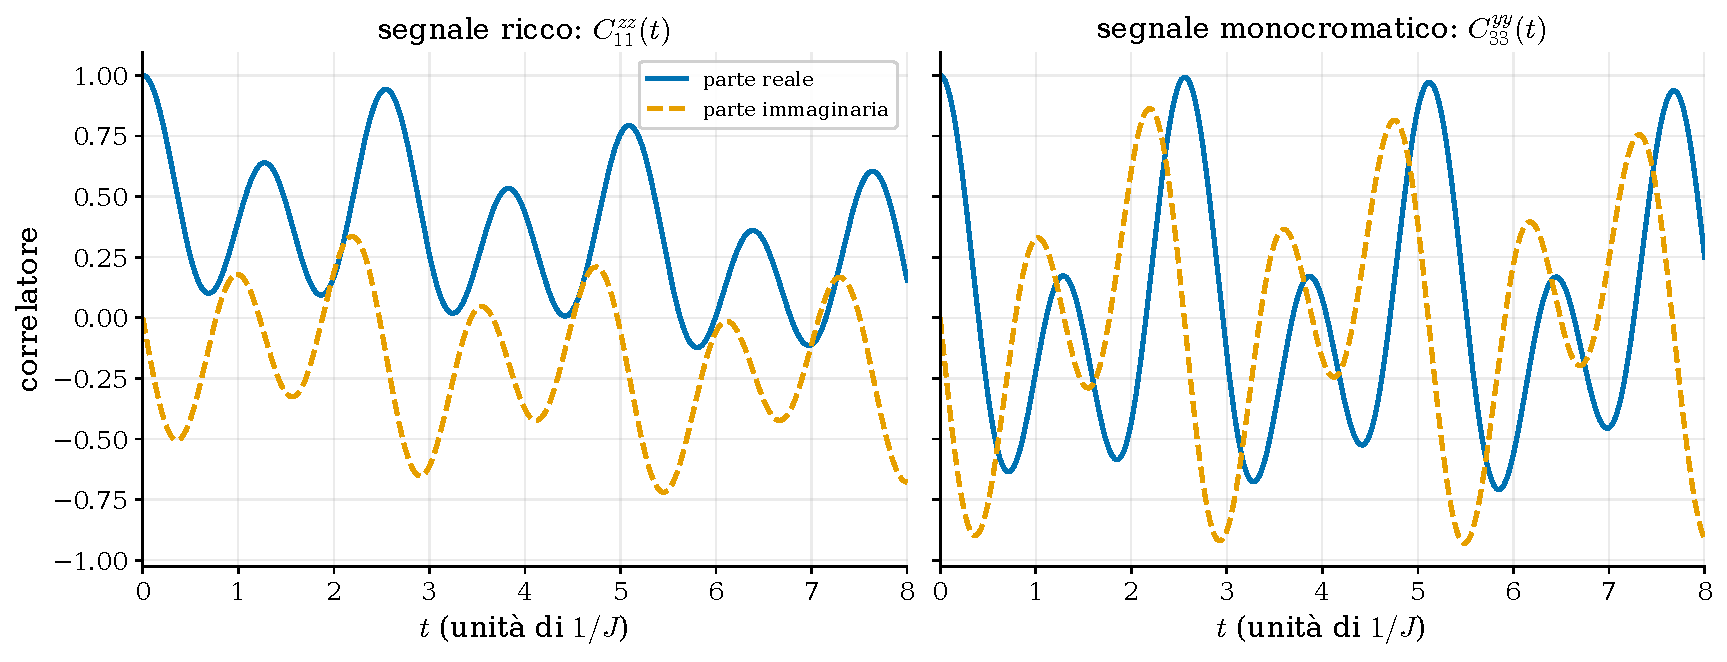
\includegraphics[width=\textwidth]{figure/fig09_ricco_piatto_anello}
\caption{Due correlatori a confronto, stessi assi. \textbf{Sinistra}
($C_{11}^{zz}$): segnale con battimento irregolare, più frequenze visibili
a occhio. \textbf{Destra} ($C_{33}^{yy}$): oscillazione più regolare, quasi
periodica.}
\end{figure}
\FloatBarrier

Come sul dimero, inserendo una risoluzione dell'identità sugli autostati di
$H$ il segnale si scompone in una somma di esponenziali,
$C_{ij}^{\alpha\beta}(t)=\sum_n c_n\,e^{-i(E_n-E_0)t}$, con $n=0,\dots,7$
(otto livelli, non quattro). Il criterio di ``ricchezza'' è quanto il peso
$c_n$ è distribuito su più righe invece che concentrato su una sola.

\begin{figure}[htbp]
\centering
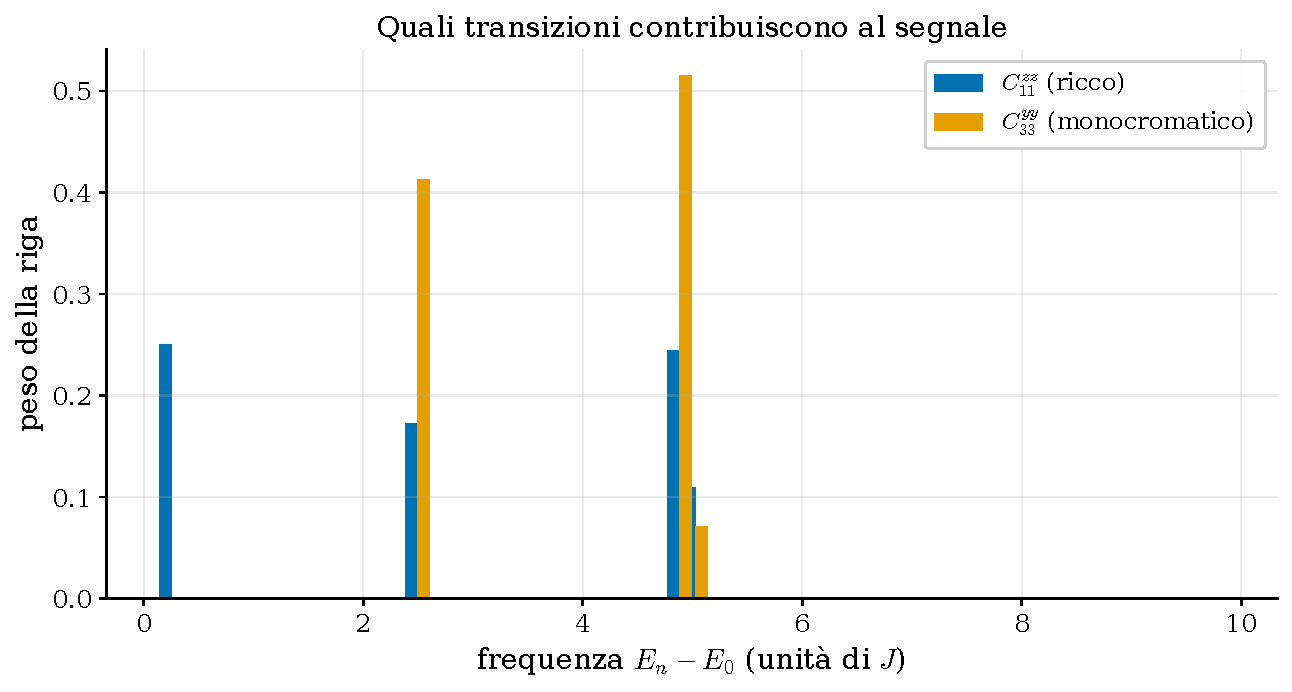
\includegraphics[width=0.76\textwidth]{figure/fig10_spettro_righe_anello}
\caption{Peso delle transizioni disponibili (esclusa $n=0$, non oscillante)
per i due correlatori della figura precedente. $C_{11}^{zz}$ distribuisce il
peso su quattro righe comparabili (concentrazione nella riga dominante:
$32\%$ del totale); $C_{33}^{yy}$ concentra il peso su due righe vicine
($52\%$ nella dominante, sul totale possibile captato da queste sei
transizioni). Entrambi condividono lo stesso insieme di frequenze --- sono
correlatori sullo stesso sito, cambia solo quali transizioni ciascuna
combinazione di componenti riesce a eccitare.}
\label{fig:spettro-righe}
\end{figure}
\FloatBarrier

\messaggio{``Ricco'' non è una proprietà della coppia di siti in sé: due
correlatori sullo stesso sito ($C_{11}^{zz}$ e $C_{33}^{yy}$, entrambi
autocorrelazioni) possono avere contenuto spettrale molto diverso, a
seconda di quali componenti di spin si perturbano e si leggono. Come sul
dimero, ampiezza e ricchezza spettrale restano proprietà indipendenti.}

\section{Quando la preparazione non è esatta}

Tutto il documento fin qui usa lo stato fondamentale esatto (ampiezze
dirette, fase fissata reale) come punto di partenza del correlatore --- non
il circuito $W$-2q.6 vero. Vale la pena chiudere il cerchio: che succede se
si prepara lo stato con l'ansatz VQE davvero, circuito completo, invece di
iniettare le ampiezze esatte?

A differenza del dimero, qui c'è un solo ansatz da confrontare, non due:
$W$-2q.6 è già l'unico candidato canonico (Documento 2), con
$\mathcal F=0.9999999999996$ a Scenario A --- praticamente esatto, non
un'approssimazione grossolana come il PMA base del dimero
($\mathcal F=0.940$). Ci si aspetta quindi un effetto piccolo, non
l'effetto marcato che il dimero mostra con il suo ansatz meno accurato.

\begin{figure}[htbp]
\centering

\includegraphics[width=\textwidth]{figure/fig_vqe_vs_esatto_correlatore}
\caption{$C_{21}^{xx}(t)$, preparazione esatta contro preparazione via
circuito $W$-2q.6, entrambe con circuito completo ($N=60$ passi di
Trotter). \textbf{Sinistra}: le due curve sono indistinguibili a questa
scala. \textbf{Destra}: lo stesso scostamento, in scala logaritmica ---
visibile solo così, ordine $10^{-7}$.}
\label{fig:vqe-vs-esatto}
\end{figure}
\FloatBarrier

\verifica{Sulla curva $C_{21}^{xx}(t)$ (13 istanti, $t\in[0,6]$): scarto
medio $2.50\times10^{-7}$, massimo $6.09\times10^{-7}$. Ripetuto
sull'intero scan delle 81 combinazioni (a $t=2$, $N=60$): scarto medio
$2.90\times10^{-7}$, massimo $1.02\times10^{-6}$ (combinazione
$C_{11}^{zz}$), minimo $6.04\times10^{-10}$.}

\subsection*{Perché qui non c'è la stessa storia ricco/monocromatico del dimero}

Sul dimero, l'errore di preparazione (fidelity $0.940$ per l'ansatz base)
si propaga in modo diverso a seconda del correlatore --- abbastanza grande
da mostrare una struttura interpretabile (scarto $0.607$ per un
correlatore, $0.019$ per un altro con l'ansatz migliore). Qui l'errore di
partenza è quasi sedici ordini di grandezza più piccolo
($1-\mathcal F\sim4\times10^{-13}$), e lo scarto propagato resta
uniformemente minuscolo: nessuna correlazione misurabile fra lo scarto e
l'ampiezza del correlatore (coefficiente di correlazione $-0.02$ su tutte
le 81 combinazioni) --- a questa scala, l'imperfezione si comporta più
come rumore numerico distribuito a caso che come un effetto strutturato da
spiegare.

\messaggio{Non è una sezione ``vuota'' perché l'effetto è piccolo: è la
conferma diretta che, a differenza del dimero, l'ansatz canonico
dell'anello non introduce nessun errore di preparazione degno di nota nella
pipeline dei correlatori --- un fatto verificato, non assunto dal solo
valore della fidelity.}

\section{Che cosa manca, dichiarato}

\begin{itemize}[leftmargin=1.5em,itemsep=2pt]
\item Tutto qui è a simulazione ideale: nessun rumore di gate, nessun
errore di lettura, ancilla letta sul vettore di stato esatto.
\item Il circuito dei correlatori resta il più lungo di questo pacchetto
--- registro a tre qubit più ancilla, $N$ passi di Trotter (Documento 3,
già il più costoso della serie) più le porte controllate: è il candidato
naturale come primo banco di prova per il sistema come sistema aperto.
\end{itemize}

\end{document}
